% ============================================================
%  Matching as Design: Recovering a Causal Effect from Observational Data
% ============================================================
\documentclass[12pt, a4paper]{article}

% ----- Packages -----
\usepackage[margin=1in]{geometry}
\usepackage{amsmath, amssymb}
\usepackage{graphicx}
\usepackage{booktabs}
\usepackage{array}
\usepackage{multirow}
\usepackage{caption}
\usepackage{subcaption}
\usepackage{hyperref}
\usepackage{xcolor}
\usepackage{float}
\usepackage{enumitem}
\usepackage{parskip}
\usepackage{titlesec}
\usepackage{fancyhdr}
\usepackage{natbib}
\usepackage{listings}

% ----- Hyperref setup -----
\hypersetup{
    colorlinks = true,
    linkcolor  = blue!60!black,
    citecolor  = blue!60!black,
    urlcolor   = blue!60!black,
}

% ----- Header / Footer -----
\pagestyle{fancy}
\fancyhf{}
\rhead{Causal Inference}
\lhead{Matching as Design}
\rfoot{\thepage}

% ----- Section formatting -----
\titleformat{\section}{\large\bfseries}{}{0em}{\thesection\quad}[\titlerule]
\titleformat{\subsection}{\normalsize\bfseries}{}{0em}{\thesubsection\quad}

% ----- Code listing style -----
\lstdefinestyle{Rstyle}{
    language        = R,
    basicstyle      = \ttfamily\footnotesize,
    keywordstyle    = \color{blue!70!black}\bfseries,
    commentstyle    = \color{gray}\itshape,
    stringstyle     = \color{orange!80!black},
    backgroundcolor = \color{gray!8},
    frame           = single,
    framerule       = 0.4pt,
    rulecolor       = \color{gray!40},
    breaklines      = true,
    numbers         = left,
    numberstyle     = \tiny\color{gray},
    xleftmargin     = 2em,
    framexleftmargin= 1.5em,
    captionpos      = b,
}
\lstset{style=Rstyle}

% ----- Placeholder box for figures -----
\newcommand{\figplaceholder}[2]{%
  \begin{figure}[H]
    \centering
    \fbox{\begin{minipage}{0.85\linewidth}
      \centering\vspace{2cm}
      {\large\color{gray} [FIGURE PLACEHOLDER]}\\[6pt]
      {\normalsize\color{gray} #1}
      \vspace{2cm}
    \end{minipage}}
    \caption{#2}
  \end{figure}
}

% ============================================================
\begin{document}

% ----- Title page -----
\begin{titlepage}
  \centering
  \vspace*{2cm}
  {\Huge\bfseries Matching as Design\par}
  \vspace{0.3cm}
  {\Large Recovering a Causal Effect from Observational Data\par}
  \vspace{0.5cm}
  {\large Causal Inference\par}
  \vspace{1cm}
  {\normalsize Hazim bin Mohd Izani\par}
  \vspace{2cm}
  {\normalsize May 6, 2026\par}
  \vfill
  \rule{0.6\linewidth}{0.4pt}
\end{titlepage}

\tableofcontents
\newpage

% ============================================================
\section{Overview}
% ============================================================

The goal of this project is to apply matching on an observational study to simulate a randomized experiment, thereby enabling reliable estimation of the average treatment effect (ATE). Matching achieves this by constructing a comparison group whose covariates are similar to each other, providing quasi-randomized conditions for ATE estimation under reasonable assumptions.

We use the LaLonde dataset, a classical dataset for observational studies using matched designs \citep{lalonde1986evaluating}. The dataset records the effect of the National Supported Work (NSW) Demonstration, a subsidized job-training program, on 1978 earnings (\texttt{re78}) for diverse workers. The dataset consists of 185 treated individuals who participated in the program and 429 controls drawn from the Current Population Survey (CPS). This dataset is particularly useful for this project because a randomized evaluation of the same program was conducted in parallel, providing an experimental benchmark ATE of approximately \$1{,}794. This gives a baseline value to which our ATE estimation can be compared.

The naive difference in mean 1978 earnings between the treated and control groups is negative, which is contradictory to the expectation of the training program positively influencing job earnings. This reflects severe selection bias, given that the NSW program targeted economically disadvantaged workers who would have earned significantly less than the control units before the training. Matching is intended to correct for this bias by finding matches of control and treatment units that have similar pre-treatment covariates.

The remainder of this report is organized as follows into four parts:
\begin{enumerate}[leftmargin=2em]
  \item \textbf{Part 1}: Data description and confounder justification.
  \item \textbf{Part 2}: Propensity score estimation and overlap diagnostics.
  \item \textbf{Part 3}: Matching methods and post-matching balance diagnostics.
  \item \textbf{Part 4}: ATE estimation, sensitivity analysis, and discussion.
\end{enumerate}

% ============================================================
\section{Part 1: Data and Confounder Justification}
% ============================================================

\subsection{Dataset Description}

The LaLonde dataset is loaded using the \texttt{MatchIt} R package. It contains 614 observations of nine variables, which are shown in Table \ref{tab:variables}.

\begin{table}[H]
  \centering
  \caption{Variable descriptions in the LaLonde dataset.}
  \label{tab:variables}
  \begin{tabular}{lll}
    \toprule
    \textbf{Variable} & \textbf{Type} & \textbf{Description} \\
    \midrule
    \texttt{treat}   & Binary  & Treatment indicator (1 = NSW participant) \\
    \texttt{age}     & Numeric & Age in years \\
    \texttt{educ}    & Numeric & Years of schooling \\
    \texttt{race}    & Factor  & Race: Black, Hispanic, White \\
    \texttt{married} & Binary  & Married (1 = yes) \\
    \texttt{nodegree}& Binary  & No high-school diploma (1 = yes) \\
    \texttt{re74}    & Numeric & Real earnings in 1974 (USD) \\
    \texttt{re75}    & Numeric & Real earnings in 1975 (USD) \\
    \texttt{re78}    & Numeric & Real earnings in 1978 (USD) — \emph{outcome} \\
    \bottomrule
  \end{tabular}
\end{table}

\subsection{Summary Statistics by Treatment Group}

Table~\ref{tab:summary} reports the mean and standard deviation of each covariate, grouped by treatment assignment. Even without further analysis, it can be seen that treated individuals had, on average, lower pre-treatment earnings (\texttt{re74}, \texttt{re75}), were less likely to be married, and were more likely to lack a high-school diploma compared to controls.

\begin{table}[H]
  \centering
  \caption{Pre-matching covariate means and standard deviations by group.}
  \label{tab:summary}
  \begin{tabular}{lrrrr}
    \toprule
    & \multicolumn{2}{c}{\textbf{Treated} ($n=185$)}
    & \multicolumn{2}{c}{\textbf{Control} ($n=429$)} \\
    \cmidrule(lr){2-3}\cmidrule(lr){4-5}
    \textbf{Variable} & Mean & SD & Mean & SD \\
    \midrule
    age       & $25.82$& 7.16& 28.03& 10.79\\
    educ      & 10.35& 2.01& 10.24& 2.86\\
    married   & 0.19& 0.39& 0.51& 0.50\\
    nodegree  & 0.71& 0.46& 0.60& 0.49\\
    re74      & 2095.57& 4886.62& 5619.24& 6788.75\\
    re75      & 1532.06& 3219.25& 2466.48& 3292.00\\
    re78      & 6349.14& 7867.40& 6984.17& 7294.16
\\
    \bottomrule
  \end{tabular}
\end{table}

The naive ATE, which was computed as a simple difference in 1978 mean earnings  between the groups was $-\$8{,}498$, compared to the experimental benchmark of $\$1{,}794$. The difference of more than $\$10{,}000$ highlights the strong selection bias present in the raw comparison, motivating the need for a matched design strategy.

\subsection{Pre-Matching Balance: Standardized Mean Differences and Variance Ratios}

To quantify the degree of imbalance, we compute the Standardized Mean Difference (SMD) for each covariate, defined as:
\begin{equation}
  \text{SMD}_j = \frac{\bar{X}_{j,\text{treated}} - \bar{X}_{j,\text{control}}}
                      {\sqrt{(S^2_{j,\text{treated}} + S^2_{j,\text{control}})/2}},
  \label{eq:smd}
\end{equation}
where $\bar{X}$ denotes the group mean and $S^2$ the group variance. An absolute SMD below $0.10$ is typically considered indicative of good balance, while values above $0.25$ show substantial imbalance and unacceptable matching. We also report the Variance Ratio ($\text{VR}_j = S^2_{j,\text{treated}} / S^2_{j,\text{control}}$), which should be close to 1 for balanced groups.

\begin{table}[H]
  \centering
  \caption{Pre-matching SMDs and variance ratios.}
  \label{tab:smd-pre}
  \begin{tabular}{lrr}
    \toprule
    \textbf{Variable} & \textbf{SMD} & \textbf{Variance Ratio} \\
    \midrule
    age       & -0.242& 0.440\\
    educ      & 0.045& 0.496\\
    married   & -0.719& 0.616\\
    nodegree  & 0.235& 0.862\\
    re74      & -0.596& 0.518\\
    re75      & -0.287& 0.956\\
  \end{tabular}
\end{table}

The largest imbalances occur for prior earnings (\texttt{re74} and \texttt{re75}) and marital status (\texttt{married}), confirming that any direct comparison of the two groups without adjustment would be misleading.

\subsection{Confounder Justification}

A variable is called a confounder if it is associated with both treatment assignment and the outcome, creating effects that bias the ATE estimation if unaccounted for. The covariates in this study satisfy this criterion, which is justified below:

\begin{description}[leftmargin=2em, style=nextline]
  \item[\texttt{age}]
    Older workers may be less likely to enroll in training and have different earnings trajectories. This may come from the fact that they have fewer years of work ahead and have accumulated more knowledge.
  \item[\texttt{educ} (years of education)]
    More educated individuals may self-select out of job training and earn more regardless.
  \item[\texttt{race}]
   Structural labor market disparities affect both program enrollment and wages.
  \item[\texttt{married}]
    Marital status correlates with labor market stability and may influence program eligibility or willingness to enroll.
  \item[\texttt{nodegree} (no high-school diploma)]
    Strongly predicts both eligibility for training programs and baseline earnings capacity.
  \item[\texttt{re74}, \texttt{re75} (prior earnings in 1974 and 1975)]
    Direct measures of pre-treatment economic status. Low prior earnings predict both enrollment (programs target disadvantaged workers) and lower future earnings absent intervention.
\end{description}

% ============================================================
\section{Part 2: Propensity Score Estimation and Overlap}
% ============================================================

\subsection{Propensity Score Model}

The propensity score $e(\mathbf{x}) = \Pr(T=1 \mid \mathbf{X}=\mathbf{x})$ is the probability of receiving the treatment given pre-treatment covariates \citep{rosenbaum1983central}. Conditioning on the propensity score allows us to control for all measured confounders. Despite the method not recreating an exact randomized experiment when matching, it allows for a more reliable comparison between groups.

We estimate $e(\mathbf{x})$ using logistic regression including all six confounder groups:
\begin{equation}
  \log\!\left(\frac{e(\mathbf{x})}{1-e(\mathbf{x})}\right)
  = \beta_0 + \beta_1\,\texttt{age} + \beta_2\,\texttt{educ}
    + \beta_3\,\texttt{race} + \beta_4\,\texttt{married}
    + \beta_5\,\texttt{nodegree} + \beta_6\,\texttt{re74}
    + \beta_7\,\texttt{re75}.
\end{equation}

The estimated coefficients and their standard errors are reported in Table~\ref{tab:ps-coefs}. Race is the strongest predictor of program participation in the CPS control group, reflecting the demographic targeting of the NSW program.

\begin{table}[H]
  \centering
  \caption{Logistic regression coefficients for the propensity score model.}
  \label{tab:ps-coefs}
  \begin{tabular}{lrrrr}
    \toprule
    \textbf{Predictor} & \textbf{Estimate} & \textbf{Std. Error} & \textbf{$z$-value} & \textbf{$p$-value} \\
    \midrule
    Intercept        & $-1.663$ & $0.971$ & $-1.713$ & $0.087$ \\
    age              & $0.016$  & $0.014$ & $1.162$  & $0.245$ \\
    educ             & $0.161$  & $0.065$ & $2.477$  & $0.013^*$ \\
    race: Hispanic   & $-2.082$ & $0.367$ & $-5.669$ & $<0.001^{***}$ \\
    race: White      & $-3.065$ & $0.287$ & $-10.699$& $<0.001^{***}$ \\
    married          & $-0.832$ & $0.290$ & $-2.866$ & $0.004^{**}$ \\
    nodegree         & $0.707$  & $0.338$ & $2.095$  & $0.036^*$ \\
    re74             & $0.000$& $0.000$ & $-2.497$ & $0.013^*$ \\
    re75             & $0.000$  & $0.000$ & $1.153$  & $0.249$ \\
    \bottomrule
    \multicolumn{5}{l}{\footnotesize Significance codes: $^{***}p<0.001$, $^{**}p<0.01$, $^*p<0.05$}
  \end{tabular}
\end{table}

\subsection{Propensity Score Distribution and Overlap}

Overlap is the assumption that every unit has a nonzero probability of receiving either treatment: $0 < e(\mathbf{x}) < 1$ for all $\mathbf{x}$. Without sufficient overlap, matching cannot find valid counterparts for some treated units and the resulting ATE estimate may be extrapolated beyond the support of the data.

Figure~\ref{fig:ps-hist} displays the propensity score distributions for treated and control units in two histograms. Figure~\ref{fig:ps-box} shows side-by-side boxplots.



\begin{figure}[H]
  \centering
  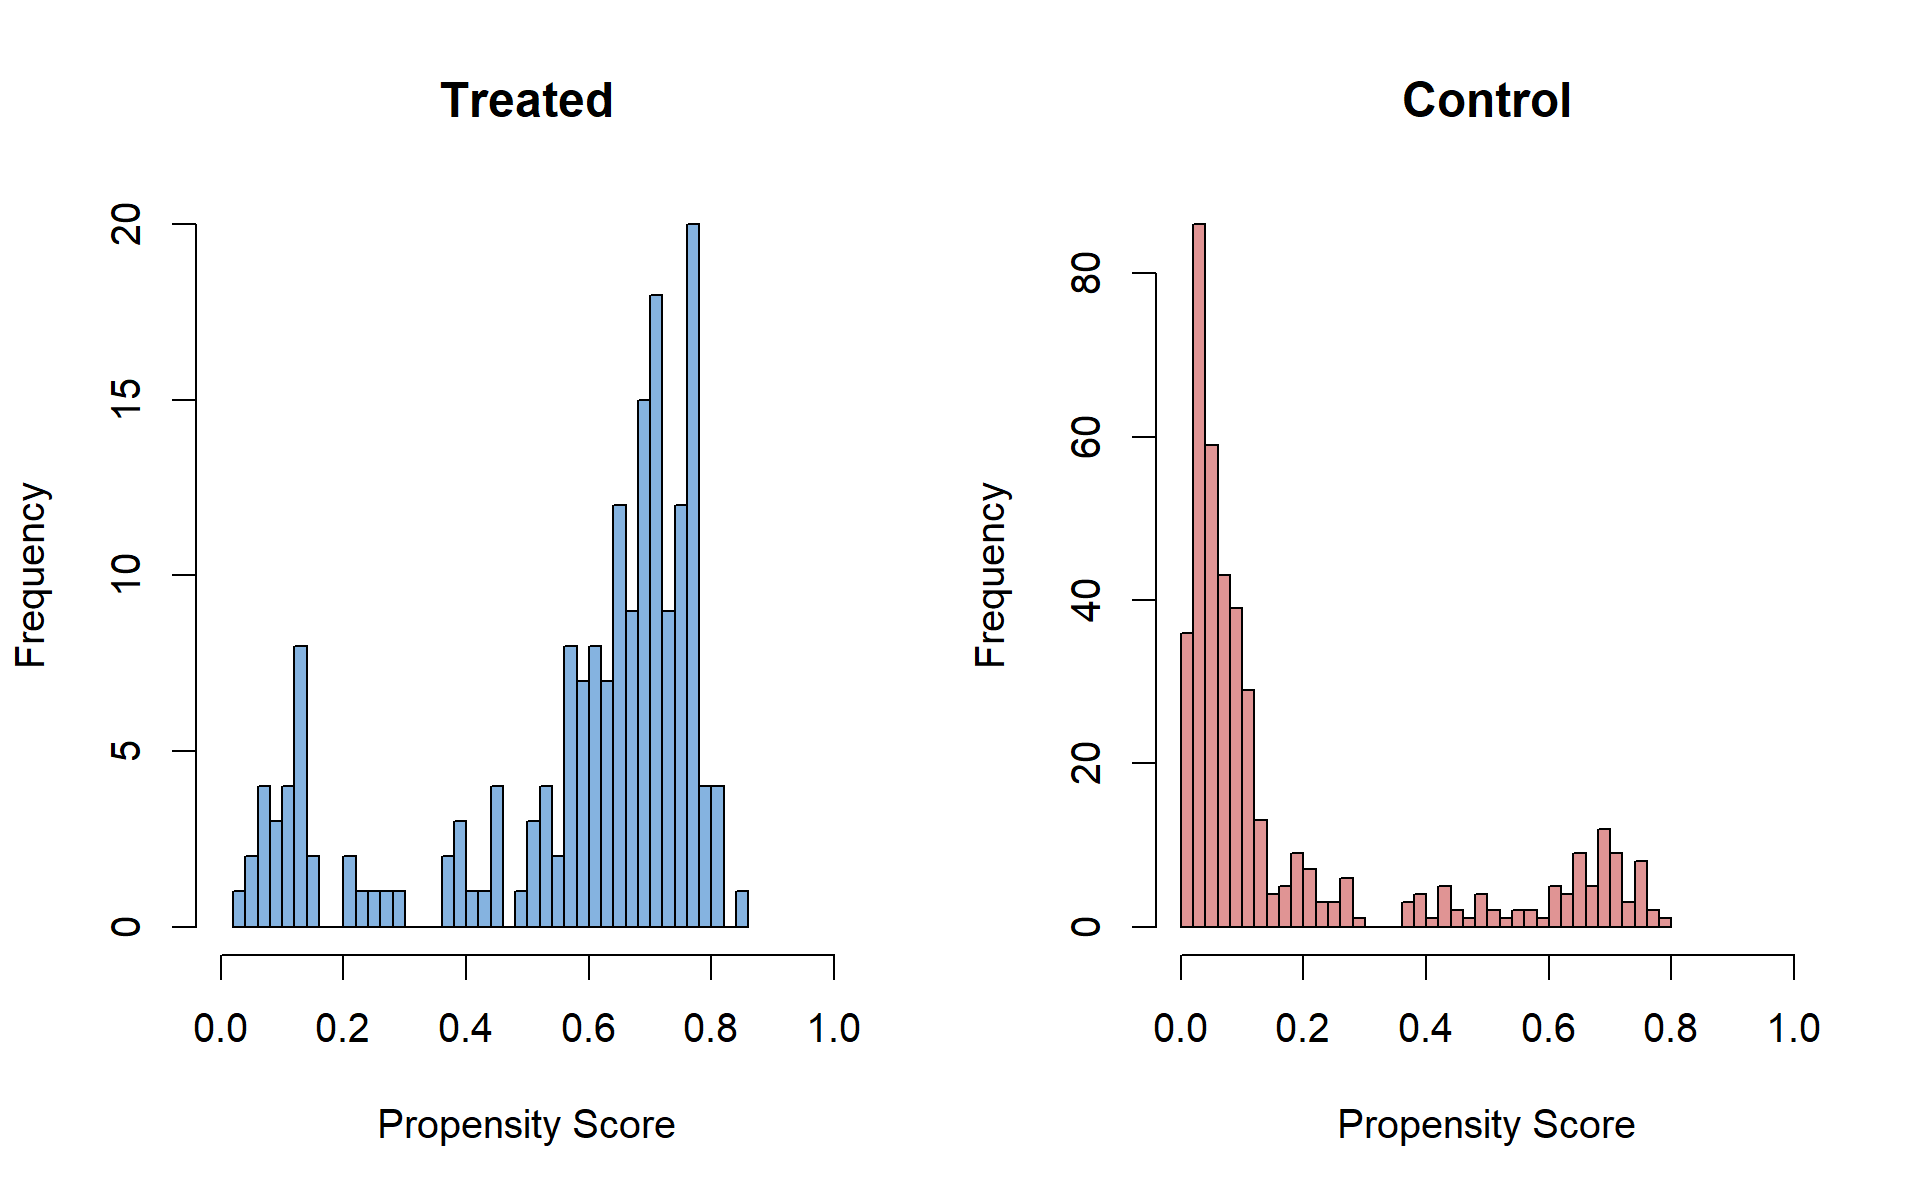
\includegraphics[width=0.85\linewidth]{images/ps_by_group.jpg}
  \caption{Propensity score distributions by treatment group.}
  \label{fig:ps-hist}
\end{figure}

\begin{figure}[H]
  \centering
  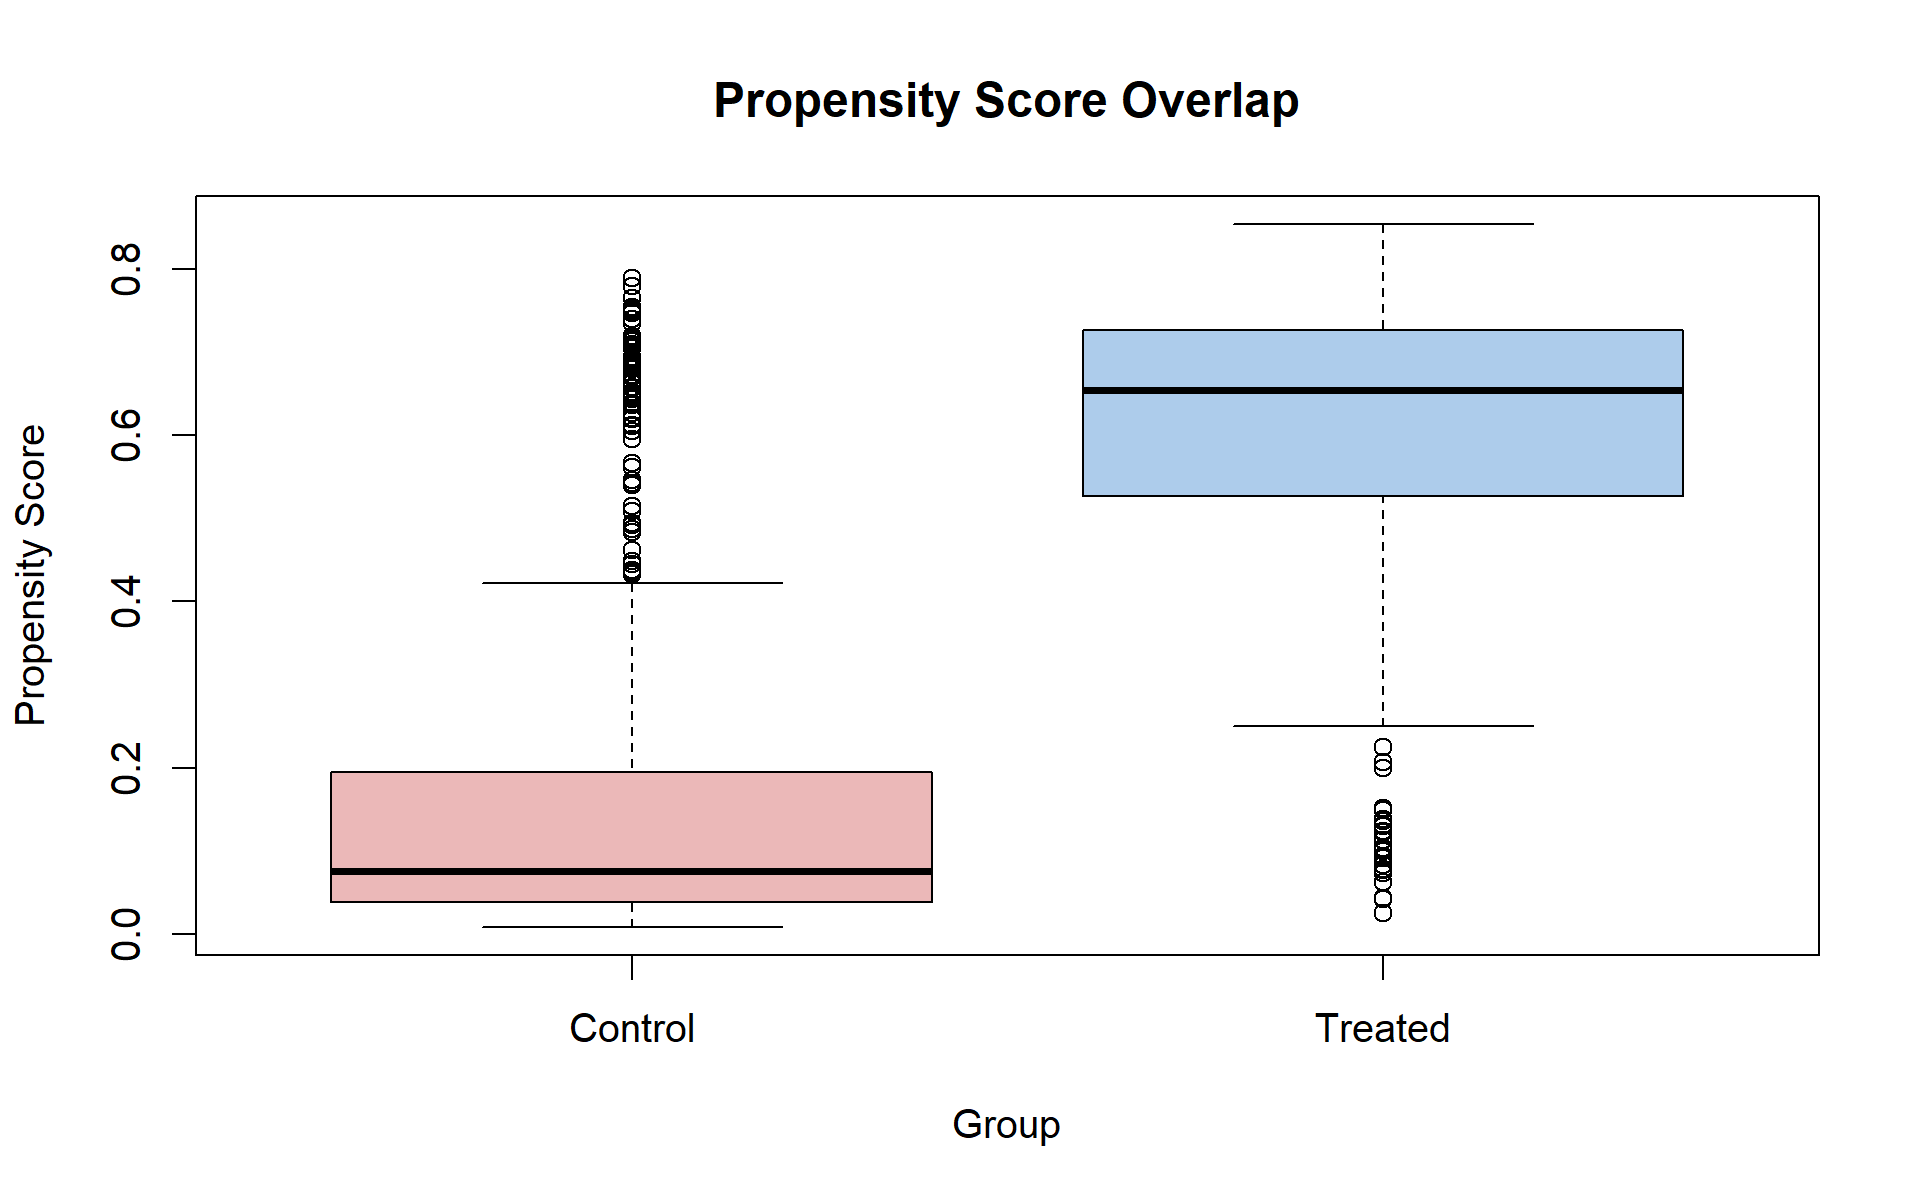
\includegraphics[width=0.85\linewidth]{images/ps_overlap.jpg}
  \caption{ Propensity score overlap: boxplots by group.}
  \label{fig:ps-box}
\end{figure}

\subsection{Overlap Statistics}

The common support region is the interval $[\max(\min e_T, \min e_C),\; \min(\max e_T, \max e_C)]$ and quantifies the range over which valid comparisons can be made. Units outside this region cannot be matched and may need to be excluded. Key statistics are:

\begin{itemize}
  \item Propensity score range for treated: $[$0.025$,$ 0.853$]$
  \item Propensity score range for control: $[$0.009$,$ 0.789$]$
  \item Common support: $[$0.025$,$ 0.789$]$
  \item Units outside common support: $65$
\end{itemize}

\subsection{Effective Sample Size under IPW}

As a supplementary diagnostic, we compute the Effective Sample Size (ESS) under Inverse Probability Weighting (IPW), which measures how many observations are effectively contributing to the estimate after reweighting:
\begin{equation}
  \text{ESS}_{\text{treated}} = \frac{\bigl(\sum_{i:T_i=1} w_i\bigr)^2}{\sum_{i:T_i=1} w_i^2},
  \qquad w_i = \frac{1}{e(\mathbf{x}_i)}.
\end{equation}
A large reduction from the nominal sample size to the ESS signals extreme weights, driven by poor overlap or propensity scores near 0 or 1.

\begin{itemize}
  \item ESS (treated): $58.3$ out of 185
  \item ESS (control): $329$ out of 429
\end{itemize}

The significant reduction in our ESS reflects the highly imbalanced propensity scores between the two groups, which was first visualized in the diagnostic plots.

\subsection{Propensity Score Distribution by Race}

Because race is the most influential predictor in the propensity score model, Figure~\ref{fig:ps-race}  shows the propensity score by race and treatment status. The strong separation between CPS whites and NSW-treated Black and Hispanic workers is the primary driver of the overall distributional imbalance observed in Section~2.2.


\begin{figure}[H]
  \centering
  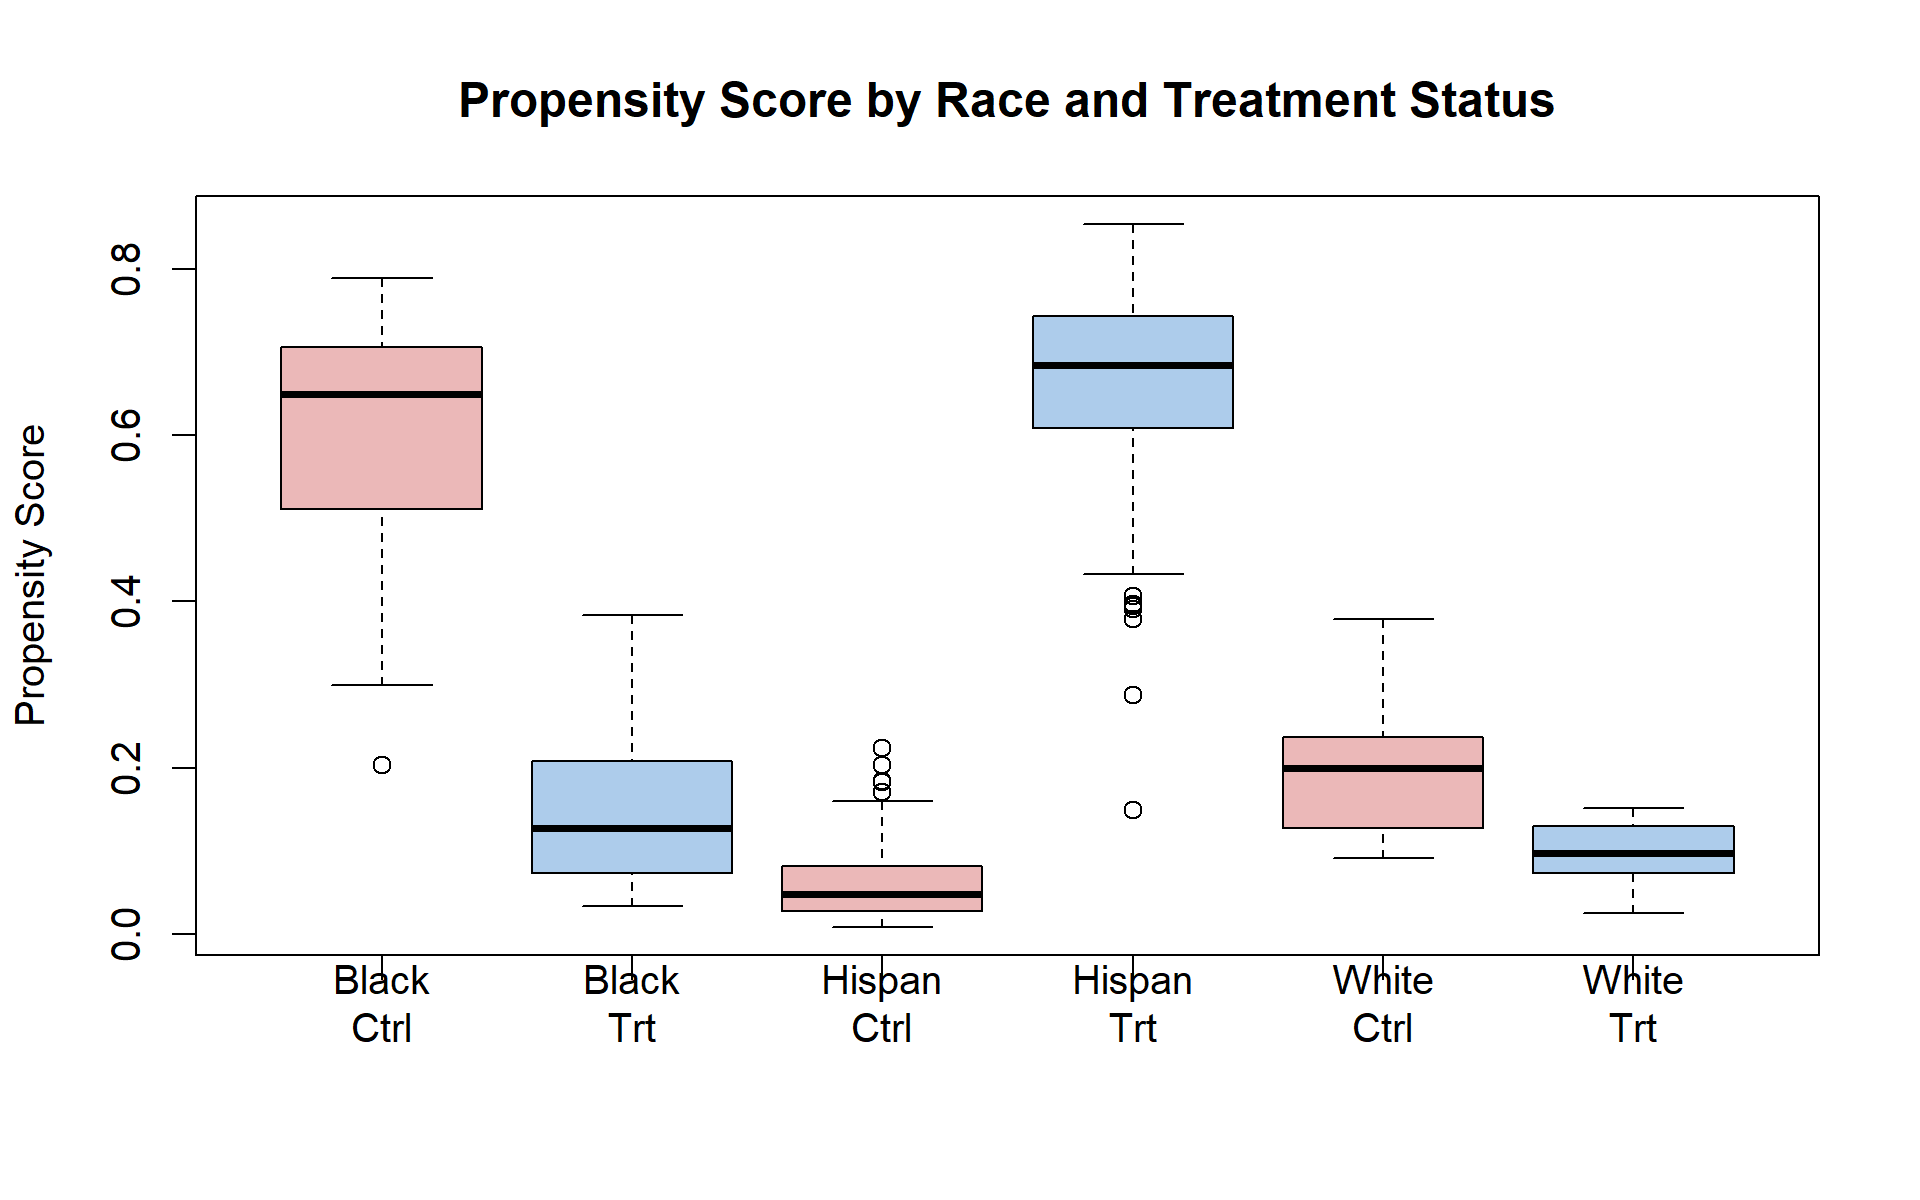
\includegraphics[width=0.85\linewidth]{images/ps_race.jpg}
  \caption{  Propensity score distribution by race and treatment status.}
  \label{fig:ps-race}
\end{figure}


% ============================================================
\section{Part 3: Matching Methods and Balance Diagnostics}
% ============================================================

We implement three matching strategies using the \texttt{MatchIt} package \citep{ho2011matchit}: (1) nearest-neighbor without a caliper, (2) nearest-neighbor with a caliper of $0.5\,\sigma_{\hat{e}}$, and (3) full matching. For each method we report balance diagnostics and the resulting matched-sample ATE.

\subsection{Nearest-Neighbor Matching Without Caliper}

\subsubsection{Method}

In 1:1 nearest-neighbor matching on the propensity score, each treated unit is paired with the control unit that has the closest propensity score. Matching is performed with no replacement or caliper, so every treated unit is matched regardless of the quality of the available match.

\subsubsection{Results}

Of the 614 observations, 244 control units were discarded, leaving 185 matched pairs (370 observations). The reduction come from the 1:1 matching scheme. Given we had 185 treated units, only 185 controls would be kept.

\begin{figure}[H]
  \centering
  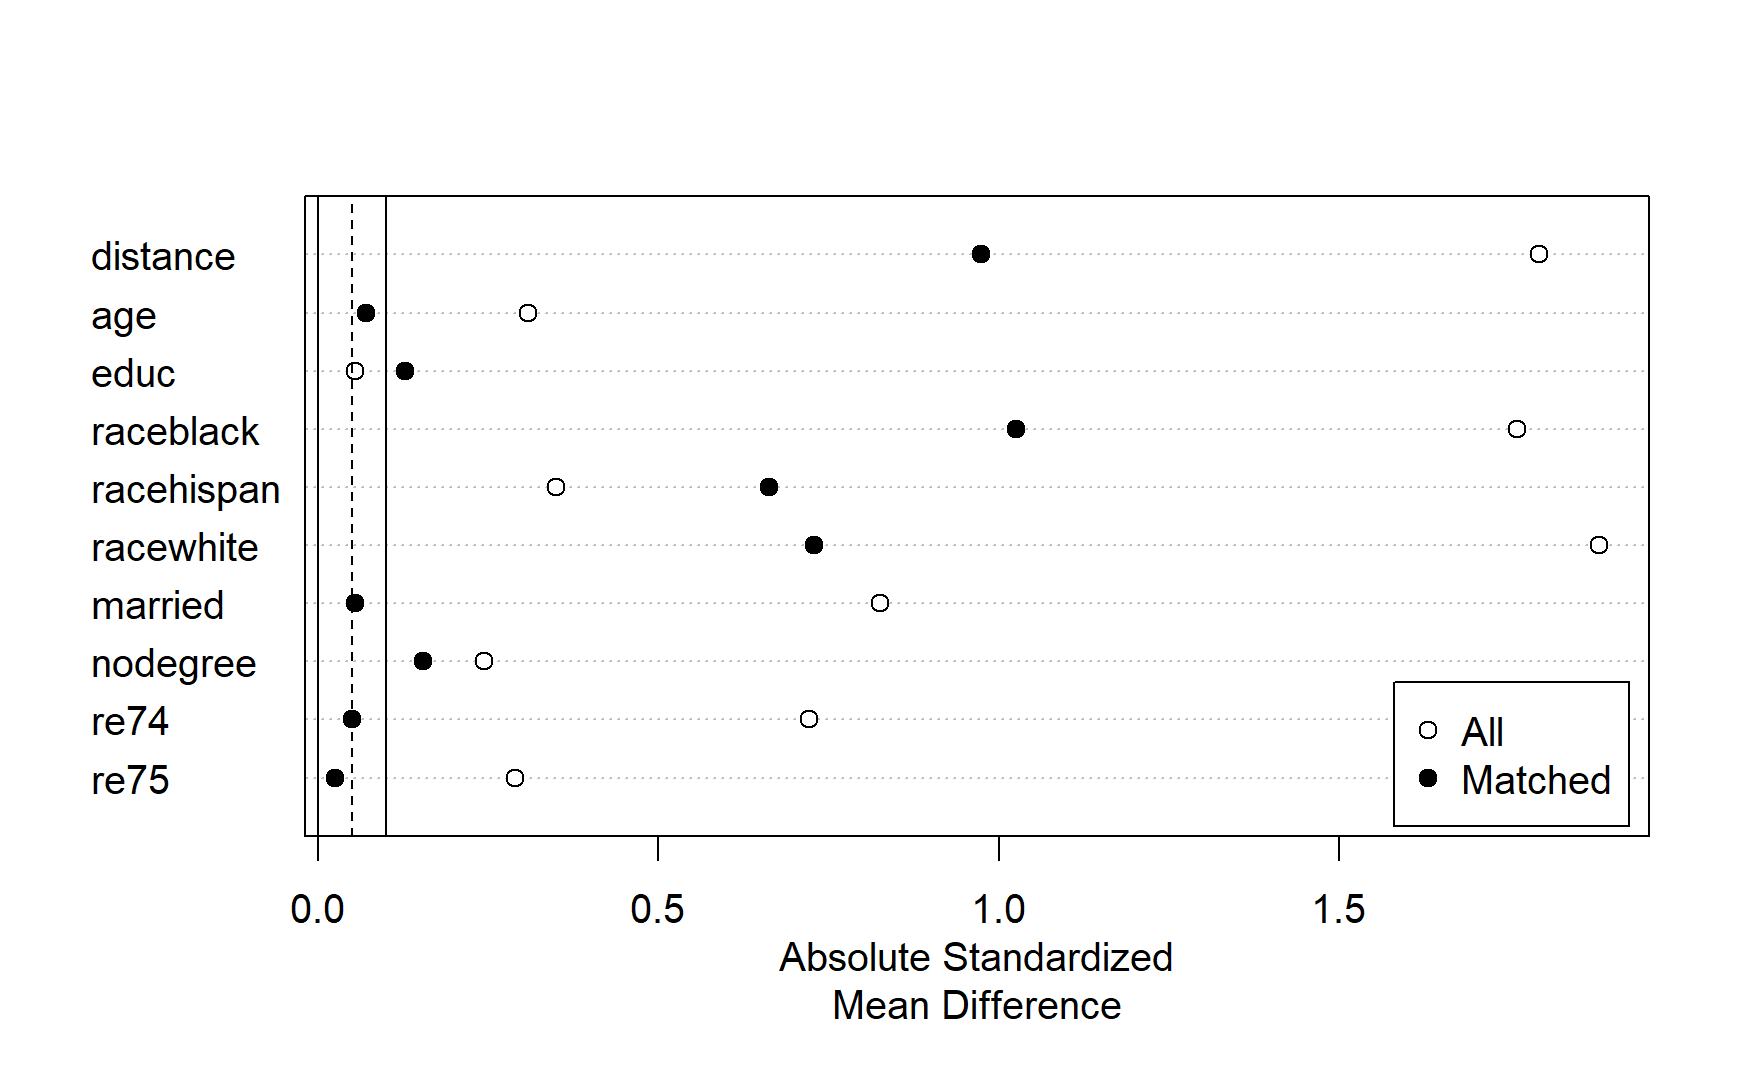
\includegraphics[width=0.85\linewidth]{images/no_caliper_love.jpg}
  \caption{Love plot: nearest-neighbor matching without caliper.}
  \label{fig:love-nn}
\end{figure}

\begin{figure}[H]
  \centering
  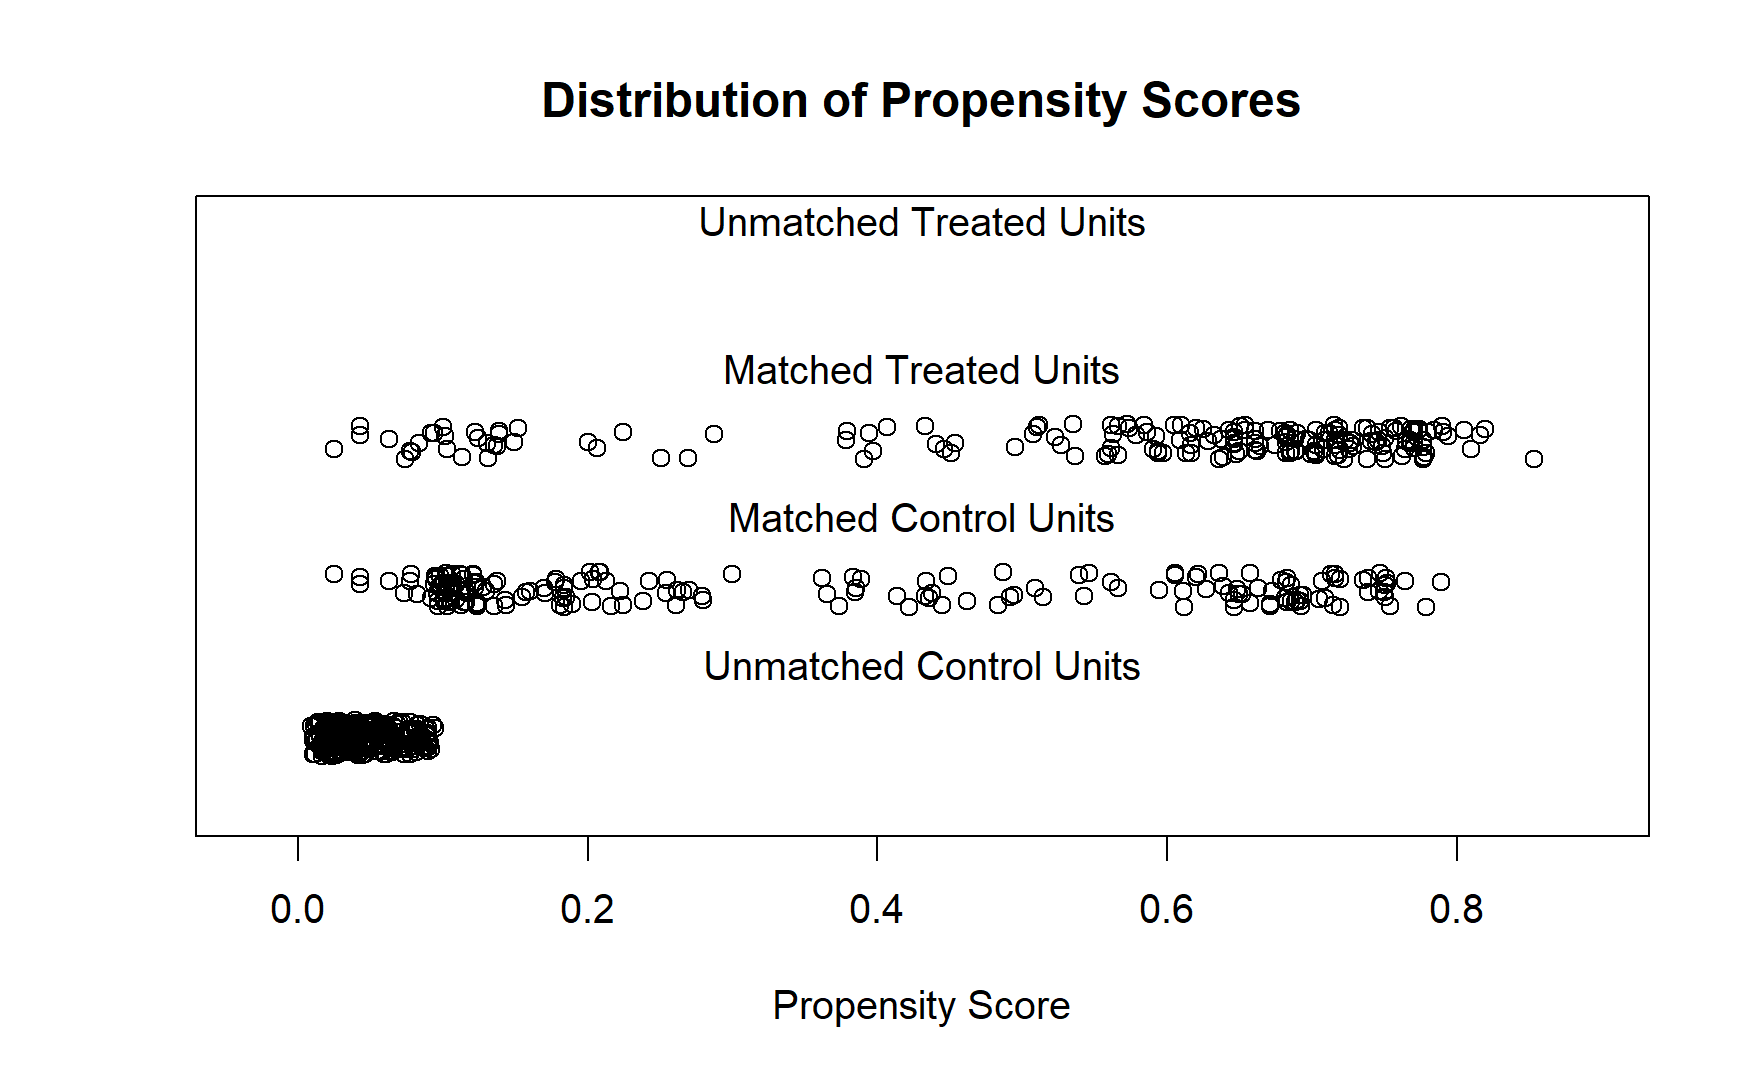
\includegraphics[width=0.85\linewidth]{images/no_caliper_dist.jpg}
  \caption{Propensity score jitter plot: NN without caliper.}
  \label{fig:jitter-nn}
\end{figure}

\begin{figure}[H]
  \centering
  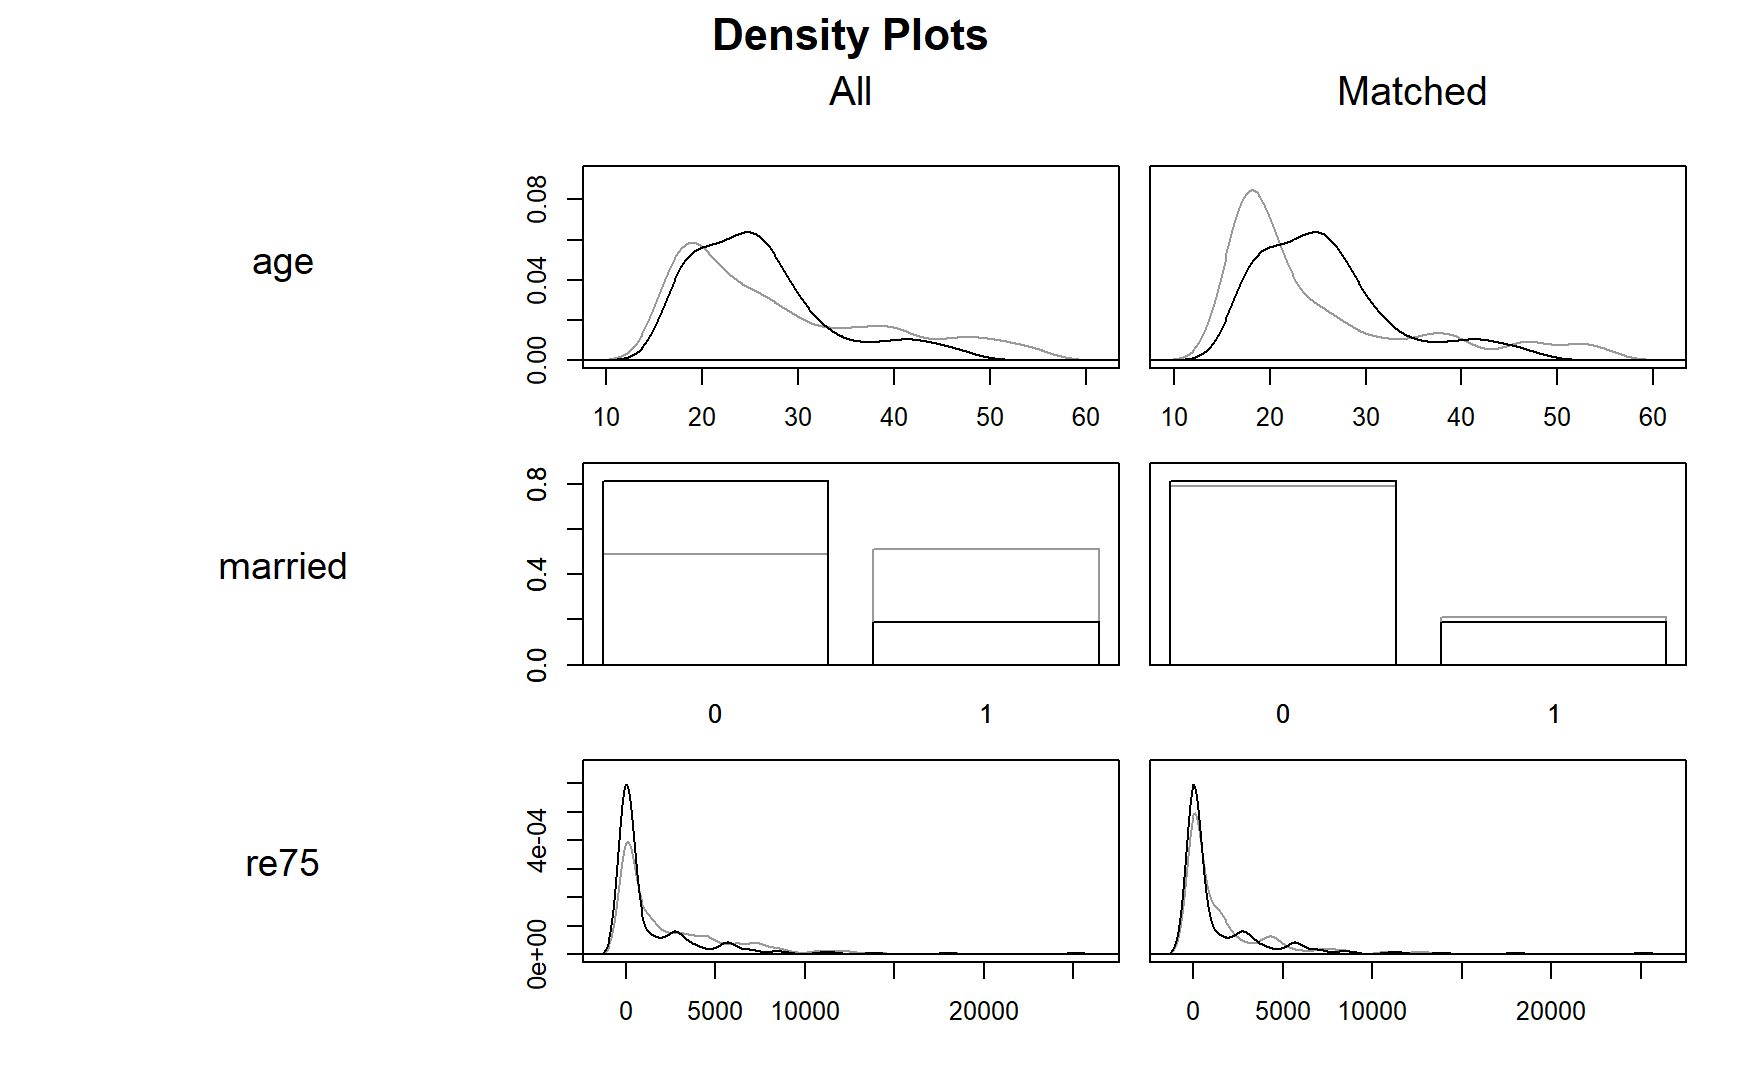
\includegraphics[width=0.85\linewidth]{images/no_caliper_density.jpg}
  \caption{Covariate density comparison: NN without caliper.}
  \label{fig:density-nn}
\end{figure}

\subsubsection{ATE Estimate}

The matched-sample ATE is computed as:
\begin{equation}
  \widehat{\text{ATE}}_{\text{NN}} = \bar{Y}_{1}^{\text{matched}} - \bar{Y}_{0}^{\text{matched}} \approx \$894.
  \label{eq:ate-nn}
\end{equation}

\paragraph{Discussion.}
The estimate of $\approx\$894$ is significantly below the experimental benchmark of $\$1{,}794$, indicating that the  nearest-neighbor design with no caliper does not fully eliminate selection bias. Without constraints on the similarity of propensity scores, some treated units are matched to controls that are actually quite far in propensity to treatment, producing matches that import residual confounding into the matched sample. The Love plot (Figure~\ref{fig:love-nn}) confirms that several covariates still exhibit $|\text{SMD}| > 0.10$ after matching.

\subsection{Nearest-Neighbor Matching With Caliper ($0.5\,\sigma_{\hat{e}}$)}

\subsubsection{Method}

A caliper imposes a maximum allowable distance between matched pairs. We use a caliper of $0.5$ standard deviations of the estimated propensity score ($\sigma_{\hat{e}}$), which was chosen arbitrarily following widely used calipers. Any treated unit for which no control lies within this range of its propensity score is left unmatched and excluded from the analysis.

\subsubsection{Results}

Imposing the caliper led to dropping 368 of the original 614, leaving 123 matched pairs (246 observations). The loss of 62 treated units reflects the small overlap in the data, where the dropped units had no counterparts that were similar enough in propensity for an adequate ATE estimation.
\begin{figure}[H]
  \centering
  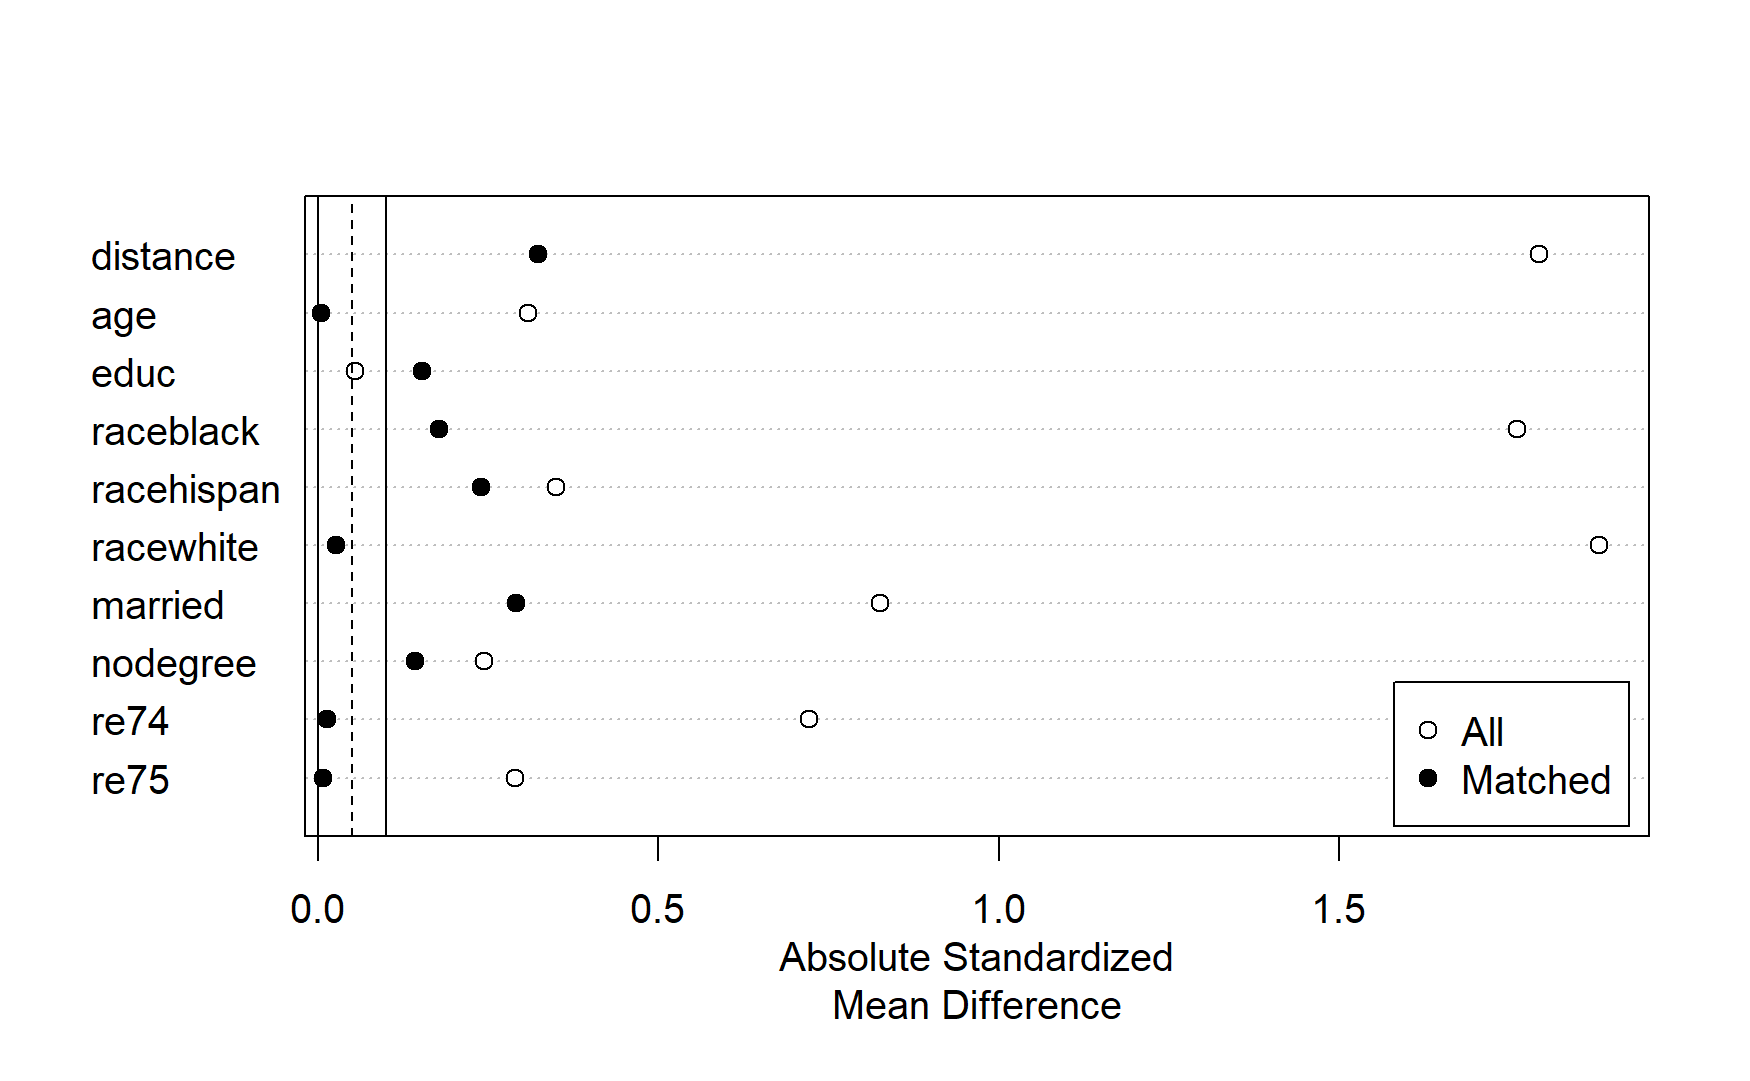
\includegraphics[width=0.85\linewidth]{images/caliper_love.jpg}
  \caption{Love plot: nearest-neighbor matching with caliper.}
  \label{fig:love-calip}
\end{figure}

\begin{figure}[H]
  \centering
  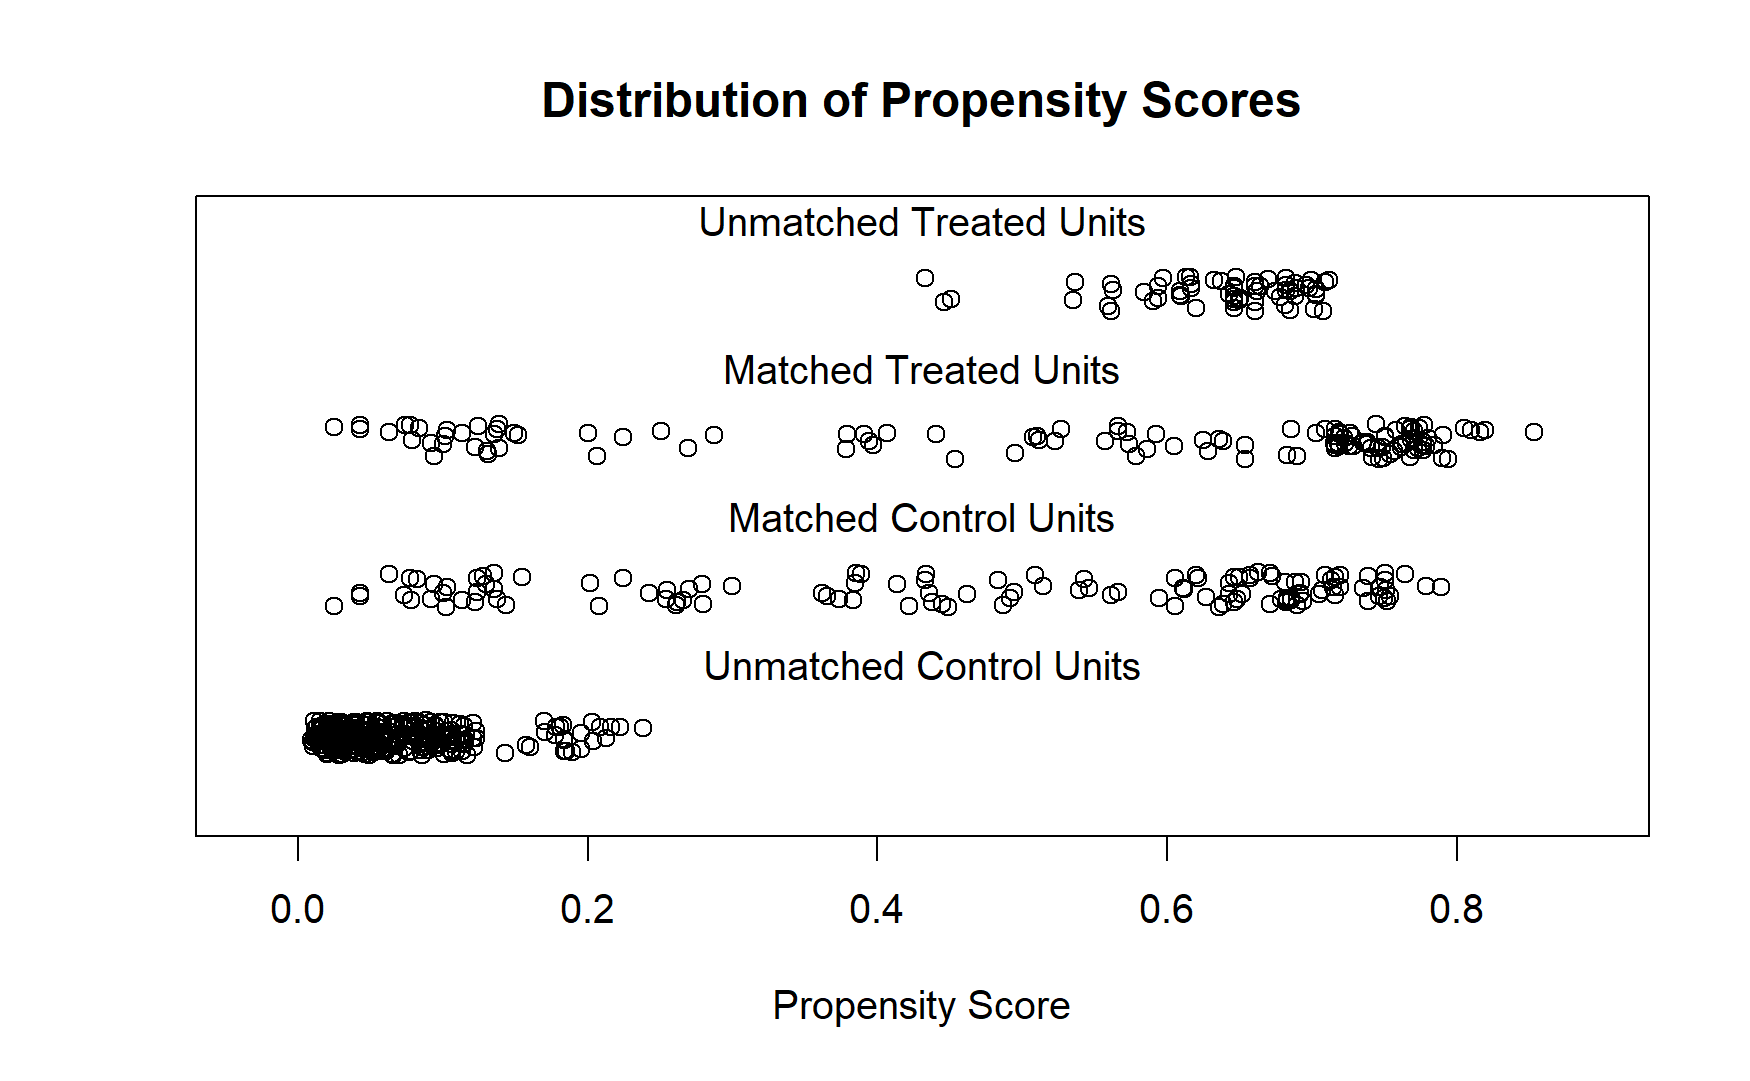
\includegraphics[width=0.85\linewidth]{images/caliper_dist.jpg}
  \caption{Propensity score jitter plot: NN with caliper.}
  \label{fig:jitter-calip}
\end{figure}

\begin{figure}[H]
  \centering
  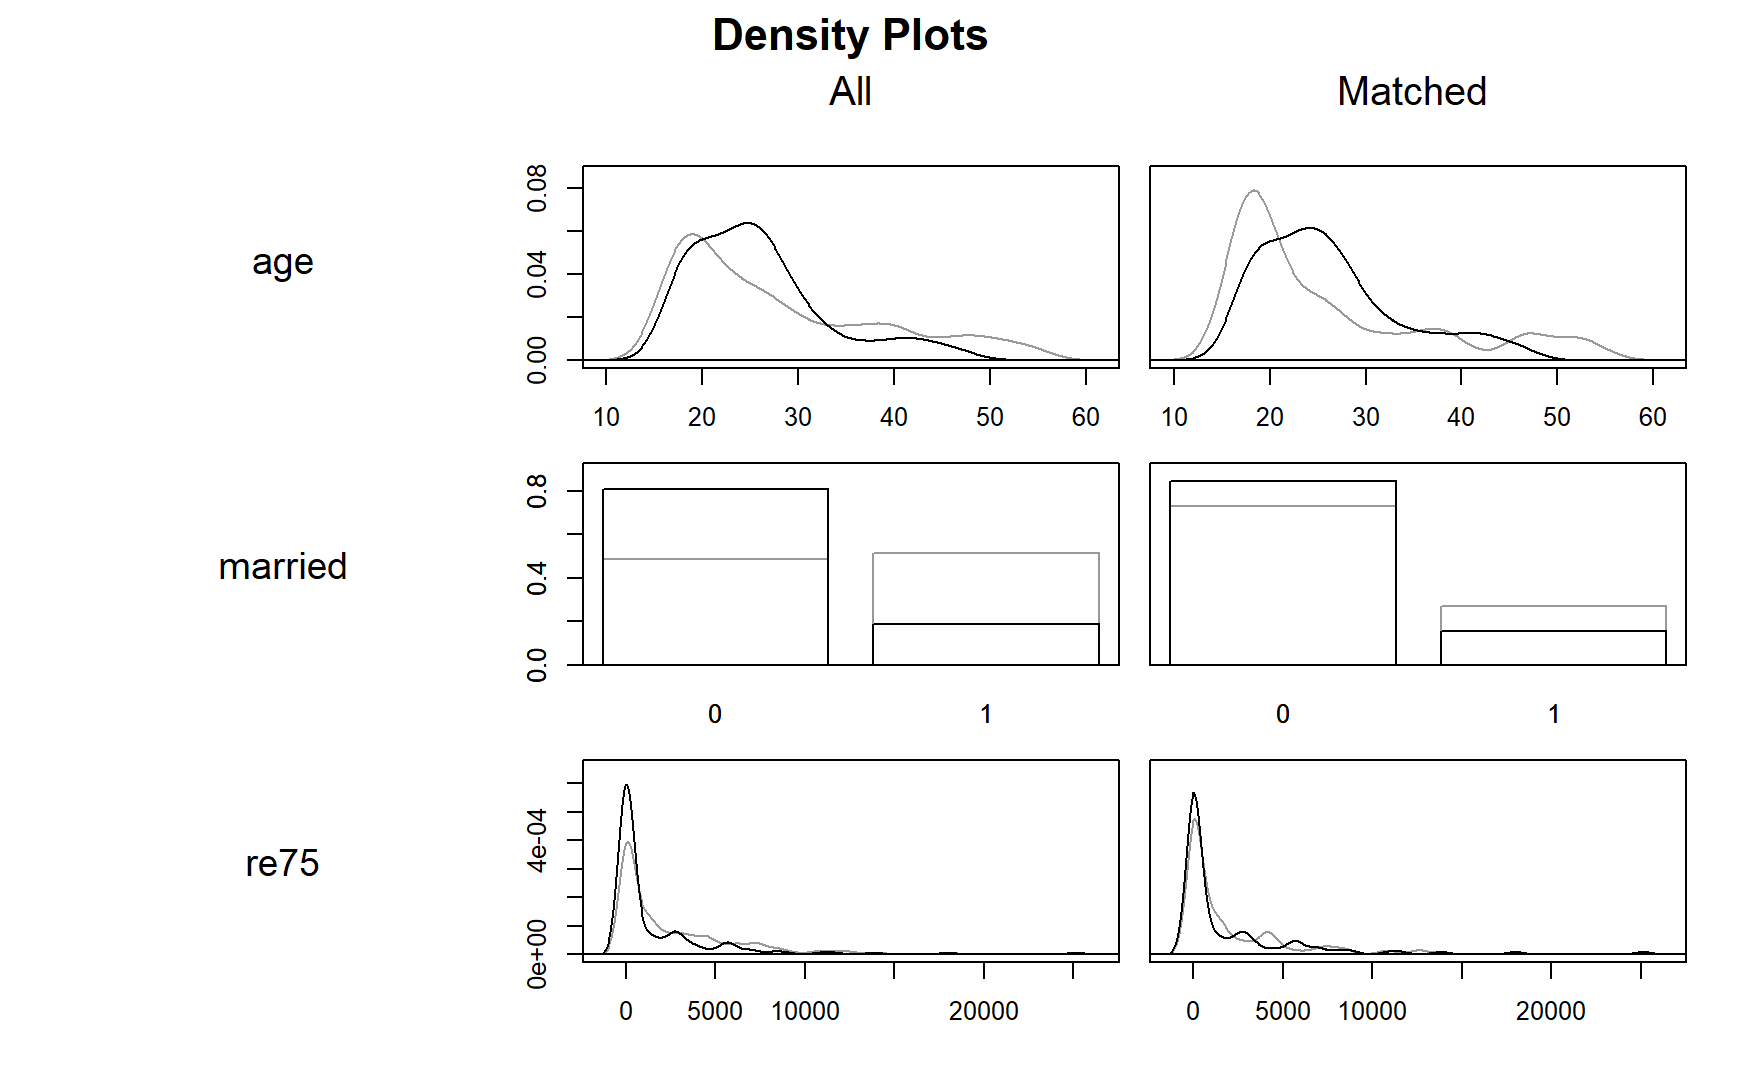
\includegraphics[width=0.85\linewidth]{images/caliper_density.jpg}
  \caption{Covariate density comparison: NN with caliper.}
  \label{fig:density-calip}
\end{figure}

\subsubsection{ATE Estimate}

\begin{equation}
  \widehat{\text{ATE}}_{\text{caliper}} \approx \$1{,}410.
  \label{eq:ate-calip}
\end{equation}

\paragraph{Discussion.}
The caliper-constrained nearest-neighbor ATE estimate of $\$1{,}410$ is considerably closer to the experimental benchmark than the uncalibrated estimate ($\$894$). One of the reasons for this improvement comes from the fact that caliper matching discards treated units with no adequate control match, reducing extrapolation and better abiding by the overlap assumption. Furthermore, the constrained matching criterion yields better covariate balance (as confirmed by the Love plot in Figure~\ref{fig:love-calip}), so the remaining matched pairs are more comparable. The trade-off is a reduction in sample size and a narrowing of the population for which the estimate is representative.

\subsection{Full Matching}

\subsubsection{Method}

Full matching \citep{rosenbaum1991characterization} partitions all observations into matched sets, each containing at least one treated and at least one control unit. Unlike 1:1 matching, full matching uses all available observations and does not discard any unit. Diverse variable set sizes are created and weighted to account for this variability. This typically achieves excellent covariate balance while retaining the full sample.

\subsubsection{Results}

All 614 observations are retained and organized into matched subclasses. Weighted balance statistics are reported in Table~\ref{tab:balance-full}.


\begin{figure}[H]
  \centering
  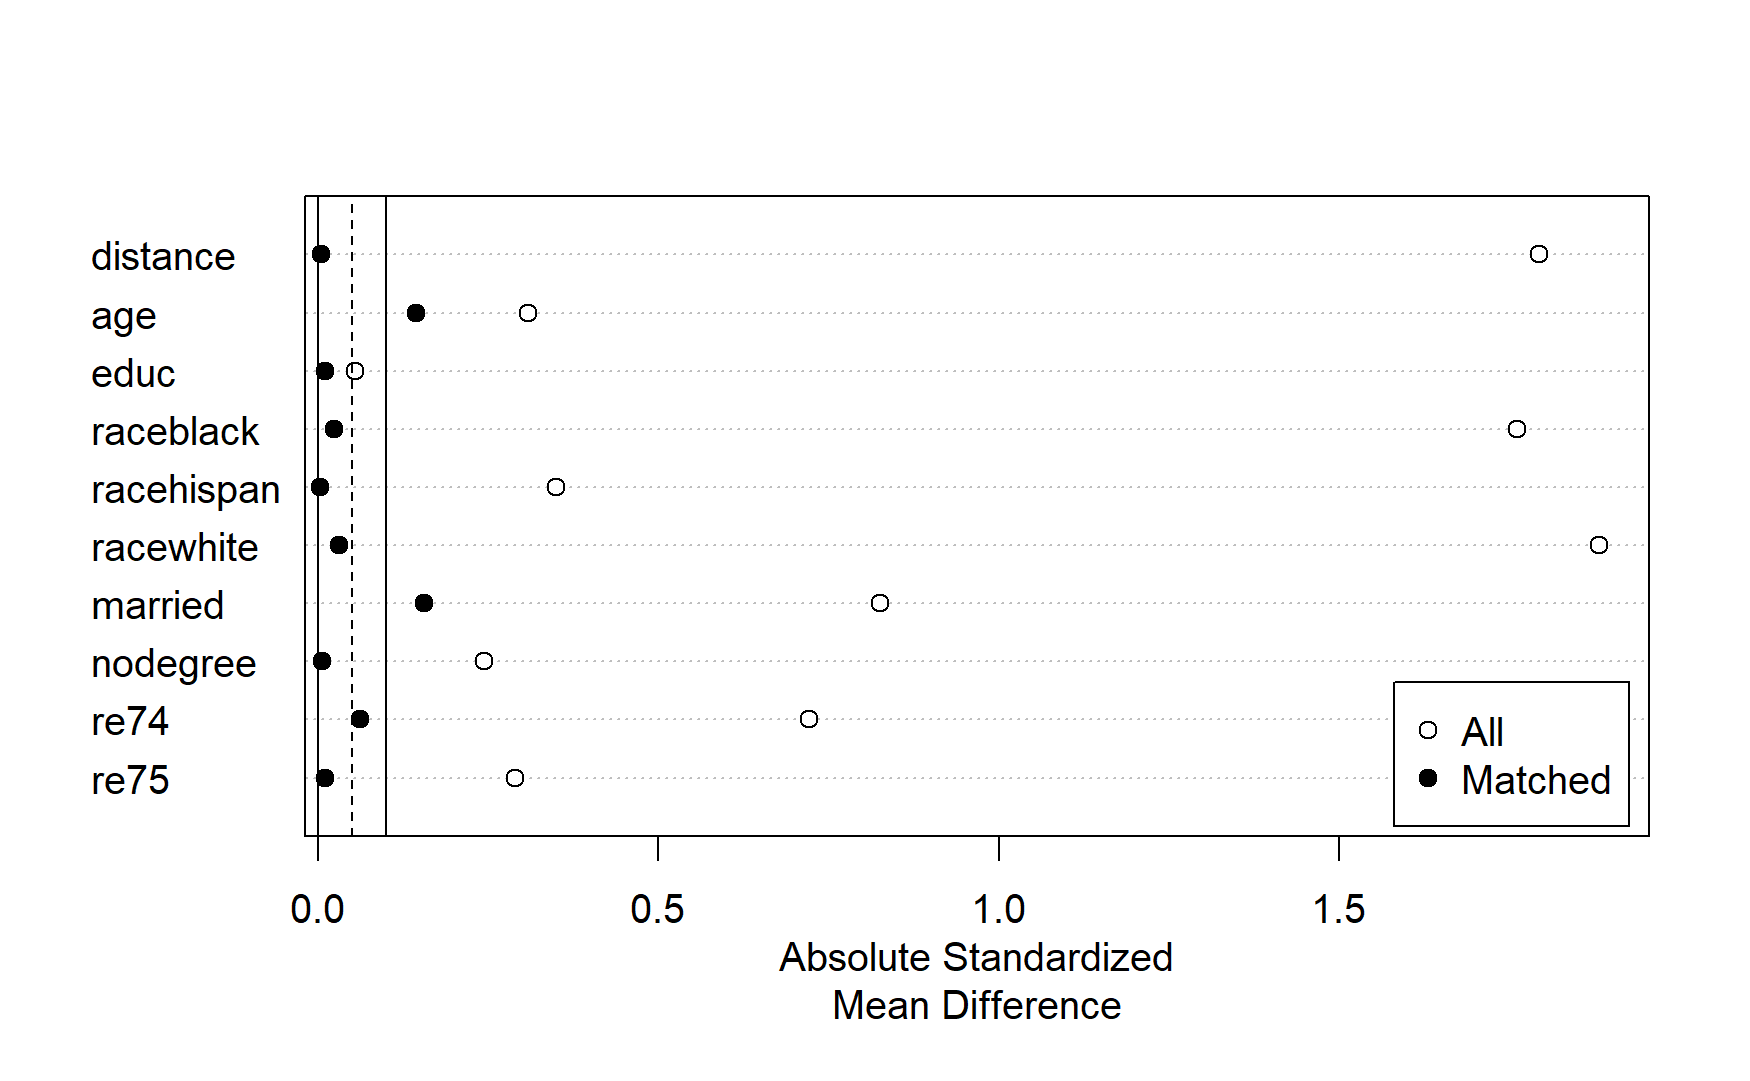
\includegraphics[width=0.85\linewidth]{images/full_love.jpg}
  \caption{Love plot: full matching.}
  \label{fig:love-full}
\end{figure}

\begin{figure}[H]
  \centering
  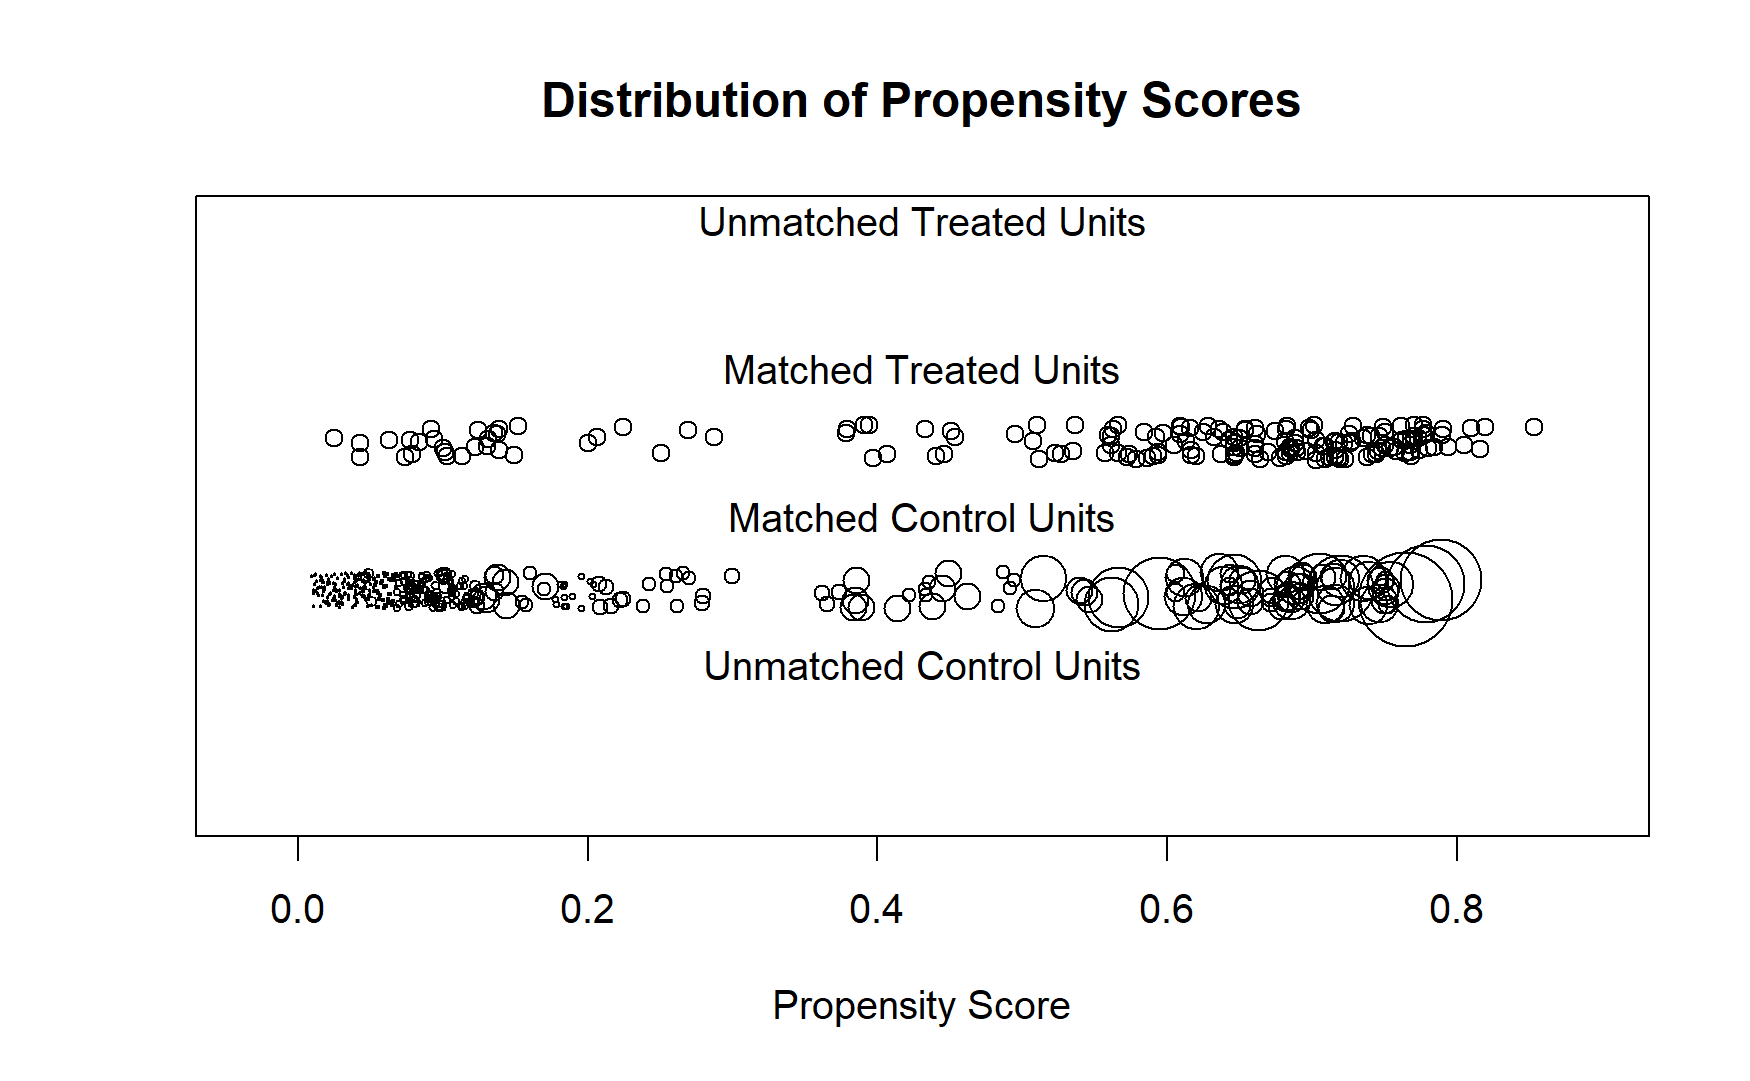
\includegraphics[width=0.85\linewidth]{images/full_dist.jpg}
  \caption{Propensity score jitter plot: full matching.}
  \label{fig:jitter-full}
\end{figure}

\begin{figure}[H]
  \centering
  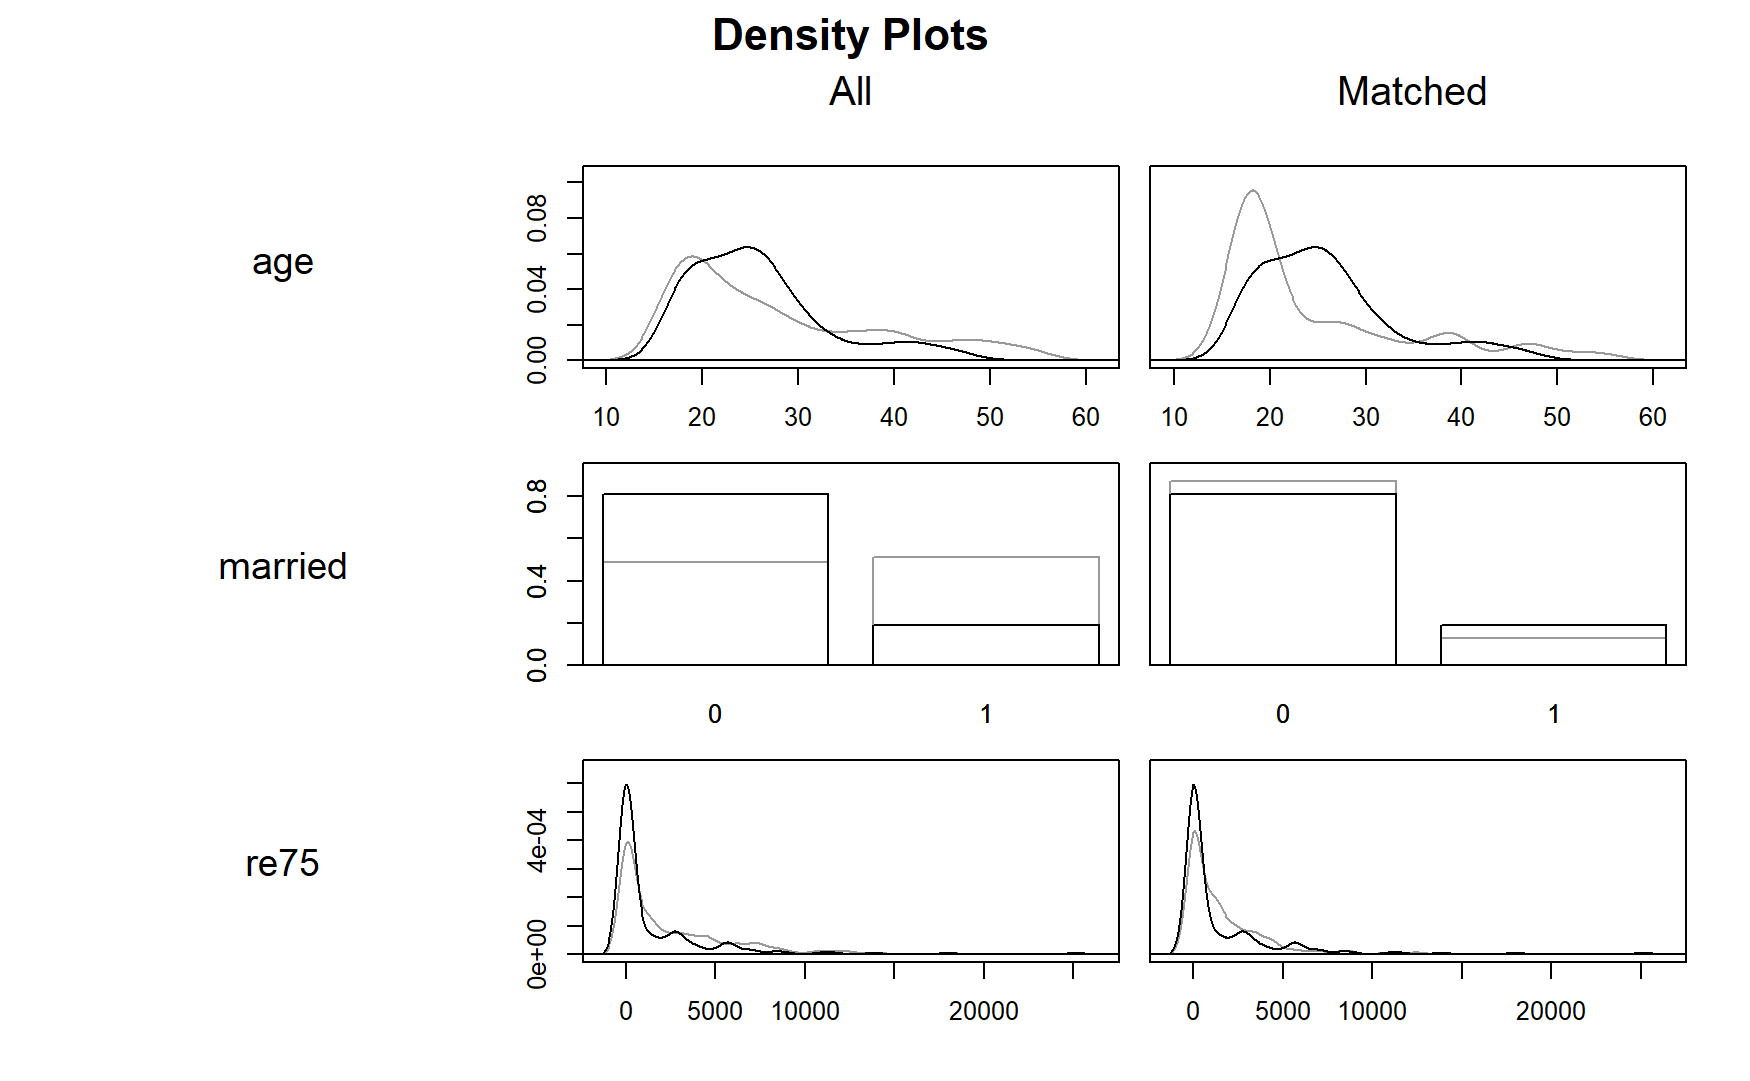
\includegraphics[width=0.85\linewidth]{images/full_density.jpg}
  \caption{Covariate density comparison: full matching.}
  \label{fig:density-full}
\end{figure}


\begin{table}[H]
  \centering
  \caption{Post-matching SMDs: comparison across methods.}
  \label{tab:balance-full}
  \begin{tabular}{lrrr}
    \toprule
    \textbf{Variable} & \textbf{NN (no caliper)} & \textbf{NN (caliper)} & \textbf{Full} \\
 & & &\\
    \midrule
    age       & 0.07& -0.01& 0.004\\
    educ      & -0.13& 0.15& -0.01\\
 raceblack& 1.03& 0.18&0.02\\
 racehispan& -0.66& -0.24&0.003\\
 racewhite& -0.73& -0.03&-0.03\\
    married   & -0.06& -0.29& 0.16\\
    nodegree  & 0.15& 0.14& -0.01\\
    re74      & -0.05& 0.01& -0.06\\
    re75      & -0.03& -0.01& -0.01\\
    \midrule
    \# matched pairs / sets & 185 & 123 & all 614 \\\end{tabular}
\end{table}

\subsubsection{ATE Estimate}

ATE estimation for full matching requires incorporating the matching weights:
\begin{equation}
  \widehat{\text{ATE}}_{\text{full}} = \sum_s \frac{n_s}{N}\,(\bar{Y}_{1s} - \bar{Y}_{0s}),
\end{equation}
where the sum runs over matched subclasses $s$, $n_s$ is the subclass size, and $N$ is the total matched-sample size.

The computed ATE was 
\[
\widehat{\text{ATE}}_{\text{full}} = \$1{,}560,
\]
which showed the best performance among the three matching schemes. One reason for this better performance is due to the corrections for extreme propensity scores conducted under full matching, which allowed for a more reasonable estimate. Furthermore, the subclasses can group multiple units to reduce the impacts of regions where there are big discrepancies of the distribution of $e(\mathbf{x})$ between treated and control groups.

% ============================================================
\section{Part 4: ATE Estimation and Discussion}
% ============================================================

\subsection{Summary of ATE Estimates}

Table~\ref{tab:ate-summary} compares all ATE estimates against the experimental benchmark.

\begin{table}[H]
  \centering
  \caption{ATE estimates by method and comparison to experimental benchmark.}
  \label{tab:ate-summary}
  \begin{tabular}{lrr}
    \toprule
    \textbf{Method} & \textbf{$\widehat{\text{ATE}}$ (USD)} & \textbf{Bias vs. Benchmark} \\
    \midrule
    Naive (no matching)& $-8{,}498$ & $-\$10{,}292$ \\
    NN without caliper          & $894$      & $-\$900$      \\
    NN with caliper ($0.5\,\sigma$) & $1{,}410$ & $-\$384$   \\
    Full matching               & $1{,}560$& $-\$234$\\
    \midrule
    \textbf{Experimental benchmark} & $1{,}794$ & --- \\
    \bottomrule
  \end{tabular}
\end{table}

\subsection{Required Assumptions}

The causal interpretation of any matched ATE rests on three key assumptions:

\begin{description}[leftmargin=2em, style=nextline]
  \item[SUTVA (Stable Unit Treatment Value Assumption)]
    Each unit's potential outcome depends only on its own treatment status. This implies that there are no interference effects and there is a single version of the treatment. For this project this means assuming there are no differences in how the training program is conducted across the treatment units and that one worker's participation does not affect another's salary.
  \item[Ignorability]
    Conditional on the observed covariates $\mathbf{X}$, treatment assignment is independent of the potential outcomes. Mathematically, we can write $(Y_0, Y_1) \perp T \mid \mathbf{X}$. Since we can't test this assumption, we would need additional background knowledge to evaluate its validity for this dataset. However, in our context, this assumption means that there are no other unmeasured confounders.
  \item[Overlap]
    Every unit has a positive probability of receiving either treatment. Mathematically, we write$0 < e(\mathbf{x}) < 1$ for all $\mathbf{x}$ in the support of $\mathbf{X}$. Violations lead to extrapolation and unreliable estimates. While we observed strong differences in the original propensity score distributions, caliper matching and full matching both mitigate this by restricting or reweighting the comparison, providing more similar propensity scores between compared units.
\end{description}

\subsection{Limitations and Discussion}

\begin{description}[leftmargin=2em, style=nextline]
  \item[Unmeasured confounders]
    Ignorability cannot be verified empirically. Factors such as motivation, geographic mobility, and access to informal networks are likely correlated with both program enrollment and future earnings but are absent from the LaLonde dataset. Sensitivity analyses (e.g., Rosenbaum bounds) can quantify how strong hidden bias would need to be to explain away the observed effect. This could be used to further understand the stability of the proposed ATE estimator.
  \item[Sensitivity to matching method]
    The three matching strategies yield noticeably different estimates (\$894 vs.\ \$1{,}410 vs.$\$1{,}560$), illustrating that the ATE estimate is not invariant to the matching design. The fundamental differences across methods justify this variability, given they represent different target populations. The full matching design showed the best performance, which also reflected on the most adequate covariate balance among the three strategies. This could be expected in this dataset, considering the significant differences in propensity scores between treated and control units, where the reweighting from full matching could mitigate the effect of extreme $e(\mathbf{x})$ values.
  \item[Generalizability]
    Caliper matching discards treated units with no close control match, narrowing inference to the sub-population for which the overlap assumption holds. Estimates are not representative of the full treated population, but refer to those within a reasonable range of overlap across the groups. This is also reflected in the reweighting promoted by full matching, prioritizing ranges with more significant overlap for estimation. Therefore, caution is needed to assess the causal effects of the training program on earnings for an arbitrary unit in the population.
\end{description}

% ============================================================
\section{Future Research and Opportunities}
% ============================================================

The following items show other ATE estimation methods that could be further tested on the LaLonde dataset. Furthermore, they highlight future tests that were not covered in this project that could better evaluate the robustness of the proposed ATE estimation method.

\begin{enumerate}[leftmargin=2em]
  \item \textbf{Mahalanobis-distance matching}: Match on the full covariate vector using Mahalanobis distance as an alternative to propensity-score matching, and compare balance and ATE recovery across methods.
  \item \textbf{Caliper sensitivity}: Examine how the caliper threshold (ranging from $0.1\,\sigma$ to $1.0\,\sigma$) affects matched-sample size, covariate balance, and ATE estimates. This would allow for evaluating $\sigma$ beyond the $0.5$ level that was used for NN matching with caliper in this project.
  \item \textbf{Rosenbaum sensitivity analysis}: Apply Rosenbaum bounds \citep{rosenbaum2002observational} to assess the robustness of the matched ATE to unmeasured confounding; specifically, determine the minimum $\Gamma$ that would render the result statistically insignificant. This could better evaluate the robustness of the estimator to unmeasured confounding, which could be present in the data.
  \item \textbf{IPW and AIPW estimates}: Compute Inverse Probability Weighted (IPW) and Augmented IPW (AIPW) estimates alongside the matching-based estimates. Given AIPW's doubly robustness, this could provide another reliable ATE estimator to be compared with the ones proposed here.
  \item \textbf{Negative control outcome test}: Regress a pre-treatment outcome (e.g., \texttt{re74}) on treatment indicator in the matched sample. Under correct matching, treatment should be uncorrelated with pre-treatment outcomes. This could be used to check for confounding, where any effect of training on \texttt{re74} should be purely due to unmeasured confounders.
\end{enumerate}

% ============================================================
% Bibliography
% ============================================================
\newpage
\bibliographystyle{apalike}
\begin{thebibliography}{9}

\bibitem[LaLonde(1986)]{lalonde1986evaluating}
LaLonde, R.~J. (1986).
\newblock Evaluating the econometric evaluations of training programs with
  experimental data.
\newblock \textit{American Economic Review}, 76(4), 604--620.

\bibitem[Rosenbaum and Rubin(1983)]{rosenbaum1983central}
Rosenbaum, P.~R., \& Rubin, D.~B. (1983).
\newblock The central role of the propensity score in observational studies for
  causal effects.
\newblock \textit{Biometrika}, 70(1), 41--55.

\bibitem[Rosenbaum(1991)]{rosenbaum1991characterization}
Rosenbaum, P.~R. (1991).
\newblock A characterization of optimal designs for observational studies.
\newblock \textit{Journal of the Royal Statistical Society: Series B}, 53(3),
  597--610.

\bibitem[Rosenbaum(2002)]{rosenbaum2002observational}
Rosenbaum, P.~R. (2002).
\newblock \textit{Observational Studies} (2nd ed.).
\newblock Springer.

\bibitem[Ho et~al.(2011)]{ho2011matchit}
Ho, D.~E., Imai, K., King, G., \& Stuart, E.~A. (2011).
\newblock MatchIt: Nonparametric preprocessing for parametric causal inference.
\newblock \textit{Journal of Statistical Software}, 42(8), 1--28.

\end{thebibliography}

\end{document}